\documentclass[a4paper,11pt]{article}
\usepackage{amsmath,amsthm,amsfonts,amssymb,amscd,amstext,vmargin,graphics,graphicx,tabularx,multicol} \usepackage[french]{babel}
\usepackage[utf8]{inputenc}  
\usepackage[T1]{fontenc} 
\usepackage[T1]{fontenc}
\usepackage{amsmath,amssymb}
\usepackage{pstricks-add,tikz,tkz-tab,variations}
\usepackage[autolanguage,np]{numprint} 
\usepackage{color}
\usepackage{ulem}

\setmarginsrb{1.5cm}{0.5cm}{1cm}{0.5cm}{0cm}{0cm}{0cm}{0cm} %Gauche, haut, droite, haut
\newcounter{numexo}
\newcommand{\exo}[1]{\stepcounter{numexo}\noindent{\bf Exercice~\thenumexo} : \marginpar{\hfill /#1}}
\reversemarginpar


\newcounter{enumtabi}
\newcounter{enumtaba}
\newcommand{\q}{\stepcounter{enumtabi} \theenumtabi)  }
\newcommand{\qa}{\stepcounter{enumtaba} (\alph{enumtaba}) }
\newcommand{\initq}{\setcounter{enumtabi}{0}}
\newcommand{\initqa}{\setcounter{enumtaba}{0}}

\newcommand{\be}{\begin{enumerate}}
\newcommand{\ee}{\end{enumerate}}
\newcommand{\bi}{\begin{itemize}}
\newcommand{\ei}{\end{itemize}}
\newcommand{\bp}{\begin{pspicture*}}
\newcommand{\ep}{\end{pspicture*}}
\newcommand{\bt}{\begin{tabular}}
\newcommand{\et}{\end{tabular}}
\renewcommand{\tabularxcolumn}[1]{>{\centering}m{#1}} %(colonne m{} centrée, au lieu de p par défault) 
\newcommand{\tnl}{\tabularnewline}

\newcommand{\trait}{\noindent \rule{\linewidth}{0.2mm}}
\newcommand{\hs}[1]{\hspace{#1}}
\newcommand{\vs}[1]{\vspace{#1}}

\newcommand{\N}{\mathbb{N}}
\newcommand{\Z}{\mathbb{Z}}
\newcommand{\R}{\mathbb{R}}
\newcommand{\C}{\mathbb{C}}
\newcommand{\Dcal}{\mathcal{D}}
\newcommand{\Ccal}{\mathcal{C}}
\newcommand{\mc}{\mathcal}

\newcommand{\vect}[1]{\overrightarrow{#1}}
\newcommand{\ds}{\displaystyle}
\newcommand{\eq}{\quad \Leftrightarrow \quad}
\newcommand{\vecti}{\vec{\imath}}
\newcommand{\vectj}{\vec{\jmath}}
\newcommand{\Oij}{(O;\vec{\imath}, \vec{\jmath})}
\newcommand{\OIJ}{(O;I,J)}

\newcommand{\bmul}[1]{\begin{multicols}{#1}}
\newcommand{\emul}{\end{multicols}}


\newcommand{\reponse}[1][1]{%
\multido{}{#1}{\makebox[\linewidth]{\rule[0pt]{0pt}{20pt}\dotfill}
}}

\newcommand{\titre}[5] 
% #1: titre #2: haut gauche #3: bas gauche #4: haut droite #5: bas droite
{
\noindent #2 \hfill #4 \\
#3 \hfill #5

\vspace{-1.6cm}

\begin{center}\rule{6cm}{0.5mm}\end{center}
\vspace{0.2cm}
\begin{center}{\large{\textbf{#1}}}\end{center}
\begin{center}\rule{6cm}{0.5mm}\end{center}
}



\begin{document}
\pagestyle{empty}
\titre{Correction du Contrôle 1 : Théorème de Pythagore, de Thalès et les fonctions }{Nom}{Prénom}{Date}{Classe}


\vspace*{0.25cm}

\exo{3} \\

\renewcommand{\arraystretch}
{3.2}

\begin{tabular}{|c|p{9cm}|p{2.5cm}|p{2.35cm}|p{2.35cm}|}
\hline 
 & \textbf{Questions} & \textbf{Réponse B} & \textbf{Réponse B} & \textbf{Réponse C} \\ 
\hline 
\textbf{1} & La notation scientifique de 1 500 000 000 est : & $1,5 \times 10^{-9}$ & $15 \times 10^{8}$ & $1,5 \times 10^{9}$ \\
\hline 
\textbf{2} & $\dfrac{5}{3}-\dfrac{1}{3} \times \dfrac{3}{2}$ est égal à : & $\dfrac{2}{3}$ & $\dfrac{7}{6}$  & 2 \\ 
\hline 
\textbf{3 }& $\dfrac{(10^{-3})^{2} \times 10^{5}}{10^{-7}}=$ & $10^{6}$ & $10^{-8}$   & $10^{-7}$ \\ 
\hline 
\end{tabular} 

\vspace*{0.5cm}


\color{red}

1) Réponse C\\

2) Réponse B\\

3) Réponse A\\





\color{black}

\exo{5} On considère la fonction suivante : $f(x)=-3x+7$ et le tableau de valeurs ci-dessous.\\

\renewcommand{\arraystretch}
{2}

\begin{tabular}{|p{1cm}|p{1cm}|p{1cm}|p{1cm}|p{1cm}|p{1cm}|p{1cm}|p{1cm}|p{1cm}|p{1cm}|}
\hline 
\textbf{x} & -3 & -2 & -1 & 0 & 1 & 2 & 3 & 4 & 5 \\ 
\hline 
\textbf{f(x)} & 16 & 13 & 10 & 7 & 4 & 1 & -2 & -5 & -8 \\ 
\hline 
\end{tabular} 

\vspace*{0.5cm}

Pour chacune des affirmations suivantes, indiquer si elle est vraie ou fausse. On rapelle que les réponses doivent être justifiées.\\

AFFIRMATION 1 : L'image de 3 par la fonction f est -2.\\

AFFIRMATION 2 : f(1) = 2\\

AFFIRMATION 3 : L'antécédent de 34 par la fonction f est -8.\\

\color{red}
AFFIRMATION 1 : On peut regarder dans le tableau de valeurs, lorsque x est égal à 3 alors f(x) vaut -2. 
ou bien on peut calculer avec l'expression littérale de la fonction f(3)=-3 x 3 + 7 = -9+7 =-2\\
C'est vrai.\\


AFFIRMATION 2 : On peut regarder dans le tableau de valeurs, lorsque x est égal à 1 alors f(x) vaut 4. 
ou bien on peut calculer avec l'expression littérale de la fonction f(1)=-3 x 1 + 7 = -3+7 =4\\
C'est Faux.\\

AFFIRMATION 3 : Pour vérifier que -8 est l'antécédent  de 34, on peut résoudre l'équation $-3x+7=34$\\

$-3x=34-7$\\
$-3x=27$\\
$x=\dfrac{27}{-3}=-9$\\

ou bien regarder si l'image de -8 est 34. $f(-8)=-3 \times (-8) +7 = 31$\\

C'est Faux.


\color{black}


\newpage

\exo{3} Voisi la représentation graphique d'une fonction k.

\begin{center}
\includegraphics[scale=1]{fonction.eps} 
\end{center}

\noindent \initq \q Déterminer graphiquement les images de 0,5 et -2,5 par la fonction k.\\

\color{red}
Par lecture graphique, l'image de 0,5 est -0,5. L'image de -2,5 par la fonction k est 2.\\


\color{black}


\q Déterminer graphiquement le ou les antécédents de -0,5.\\

\color{red}
Par lecture graphique, les antécédents de -0,5 sont -0,5 et 0,5.\\


\color{black}
\q Est-il vrai que k(-1,5) = k(1,5) ? Jusitifier votre réponse.\\

\color{red}
Par lecture graphique, on peut lire que l'image de -1,5 est 2.\\
De même, l'image de 1,5 est 2 aussi.\\
On constate donc que k(-1,5) = k(1,5).\\


\color{black}

\exo{3} Dans un coin de sa chambre mansardée, Lucie installe une étagère comme représentée sur le schéma ci-dessous. L'étagère est-elle parallèle au sol ?\\

\begin{center}

\includegraphics[scale=0.5]{recithales.eps} 
\end{center}


\color{red}
Conversions utiles : 50 cm = 0,5 m et 70 cm = 0,7 m\\

Les points A, D et B sont alignés dans le même ordre que les points A, E et C.\\

On va vérifier l'égalité de Thalès :\\

D'une part, $\dfrac{\textcolor{green}{AD}}{\textcolor{red}{AB}}=\dfrac{2}{2,5}=\dfrac{20}{25}=\dfrac{4}{5}=\dfrac{124}{155}$\\

D'autre part, $\dfrac{\textcolor{green}{AE}}{\textcolor{red}{AC}}=\dfrac{2,4}{3,1}=\dfrac{24}{31}=\dfrac{120}{155}$\\

On constate que $\dfrac{AD}{AB} \ne \dfrac{AE}{AC}$, donc d'après la contraposé du  théorème de Thalès, les droites (MP) et (KL) ne sont pas parallèles. L'étagère n'est donc pas parallèle au sol.\\

\color{black}

\newpage

\exo{6} 
Des élèves participent à une course à pied.\\
Avant l'épreuve, un plan leur a été remis.
Il est représenté par la figure ci-contre.\\
On convient que :\\
- Les droites (AE) et (BD) se coupent en C.\\
- Les droites (AB) et (DE) sont parallèles.\\
- ABC est un triangle rectangle en A.

\begin{center}
\includegraphics[scale=0.6]{thalesbrevet.eps} 
\end{center}

$\rightarrow$ \textbf{ Calculer la longueur réelle du parcours ABCDE.}\\

\color{red}
Pour calculer la longueur du parcours, il nous manque les longueurs BC, CD et DE.\\

\textbf{- Calcul de la longueur BC :}\\

Dans le triangle ABC rectangle en A, l'hypoténuse est le côté [BC].\\

D'après le théorème de Pythagore, on a : \hspace*{1cm} $BC^{2}=AB^{2}+AC^{2}$\\

On remplace par les valeurs : $BC^{2}=300^{2}+400^{2}$\\

Donc  $BC^{2}=90 000+160 000$\\

 $BC^{2}=250 000$\\
 
  Ainsi  $BC= \sqrt{250 000}=500 m$\\ 


\textbf{- Calcul des longueurs CD et DE :}\\



Dans les triangles ABC et CDE :
\bi
\item Les droites (BD) et (AE) sont sécantes en C.
\item (AB) $\slash\slash$ (DE)
\ei

D'après le théorème de Thalès, on a:

\begin{center}
$\dfrac{\textcolor{green}{BC}}{\textcolor{red}{CD}}=\dfrac{\textcolor{green}{AC}}{\textcolor{red}{CE}}=\dfrac{\textcolor{green}{AB}}{\textcolor{red}{DE}}$\\
\end{center}
 



On remplace : \hspace*{1cm} $\dfrac{500}{CD}=\dfrac{400}{1000}=\dfrac{300}{DE}$\\


\textbf{Calcul de CD :}\\

$\dfrac{500}{CD}=\dfrac{400}{1000}$ donc $CD = \dfrac{500 \times 1000}{400}$\\

\fbox{CD = 1 250 m} \\

\textbf{Calcul de DE :}\\

$\dfrac{400}{1000}=\dfrac{300}{DE}$ donc $DE = \dfrac{300 \times 1000}{400}$\\

\fbox{ED = 750 m} 

La longueur du parcours totale est donc égale à 1 250 + 750 + 500 + 300 = 2 800m.\\

\color{black}


\end{document}
